\subsection*{Experiment 8.24 \quad Measurement of the relation between the emergent intensity $I$ and the rotation angle $\theta$ of a ``polarised-light intensity regulator''}

Light is an electromagnetic wave; its electric and magnetic field vectors are mutually perpendicular and both are perpendicular to the direction of propagation. The electric vector is usually taken to represent the light vector. In a plane perpendicular to the direction of propagation the light vector may assume various states of vibration, which are called the polarisation states of light. If the direction of the light vector is arbitrary and the average magnitude of the light vector is the same in every direction, the light is called natural light. If the direction of the light vector remains unchanged and only its amplitude varies with phase, so that the end point of the light vector traces out a straight line, the light is called linearly polarised light or plane-polarised light. A device that can convert natural light into polarised light is called a polariser; a device used to test whether light is polarised is called an analyser. Polariser and analyser are collectively called polarising plates. Consider a beam of natural light passing through two polarising plates set at a certain angle $\theta$ to each other; the emergent intensity and the angle $\theta$ satisfy the following relation:
\[
I=DI_0\cos^n\theta,
\]
where $I_0$ is the intensity of the polarised light incident on the analyser, which has a definite value once the apparatus is fixed, $D$ is the light transmission coefficient of the analyser, and $n$ is a coefficient to be determined. Using the apparatus provided, measure the relation between $I$ and $\theta$, and obtain the above relation by curve fitting.

\textbf{[Apparatus and materials available]} Two polarising plates with graduated discs, optical bench, one laser and its power supply, optical power meter with a silicon photocell, graph paper, etc.

\textbf{[Requirements]}

(1) The direction of the optic axis of a polarising plate is not necessarily at the $0\degree$ position of its graduated disc; the directions of the optic axes of the two plates must be determined by the experimenter. (The light emitted by a semiconductor laser is partially polarised.)

(2) Draw the experimental arrangement and measure the data of the $I$--$\theta$ relation.

(3) Determine the coefficient $n$ to be found by a graphical method.

(4) Write down the functional relation between $I$ and $\theta$.

\textbf{Solution 8.24}\quad \textbf{1.} Make the laser beam pass perpendicularly through the centres of the polariser and the analyser and fall normally on the silicon photocell of the optical power meter detector. Measure the intensity $I$ with the optical power meter and read the corresponding angle $\theta$ on the graduated disc of the analyser, thus measuring the relation between $I$ and $\theta$.

\textbf{2.} Rotate the disc of the analyser slowly, that is, change the direction of the optic axis of the analyser. When the reading of the optical power meter reaches its minimum or zero, the optic axis of the analyser is perpendicular to that of the polariser. Taking logarithms of both sides of the formula $I=DI_0\cos^n\theta$ gives
\[
\ln I=\ln DI_0+n\ln\cos\theta.
\]
Plot $\ln I$ against $\ln\cos\theta$; the slope of the resulting straight line is the coefficient $n$ to be determined.

\textbf{3. Experimental data}

\begin{center}
\textbf{Table 8.24-1}\\[3pt]
\begin{tabular}{ccccccc}
\toprule
$\theta/\degree$ & 4.5 & 15.5 & 24.5 & 35.5 & 44.5 & 55.5 \\
\midrule
$I/\mathrm{mW}$ & 1.710 & 1.587 & 1.431 & 1.129 & 0.870 & 0.550 \\
\bottomrule
\end{tabular}
\end{center}

\begin{center}
\textbf{Table 8.24-2}\\[3pt]
\begin{tabular}{ccccccc}
\toprule
$\ln\cos\theta$ & $-3.09\times10^{-3}$ & $-0.0370$ & $-0.0944$ & $-0.206$ & $-0.338$ & $-0.568$ \\
\midrule
$\ln I$ & 0.536 & 0.462 & 0.358 & 0.121 & $-0.139$ & $-0.598$ \\
\bottomrule
\end{tabular}
\end{center}

A linear regression of the data in Table 8.24-2 gives the slope $n=2.007$ and the correlation coefficient $r=0.99994$. The graphical method gives the slope of the straight line as $n=2.01$, hence $n\approx2$ (the graph is omitted).

The fitted empirical formula is
\[
I=1.710\cos^2\theta\qquad(\text{unit: mW}).
\]

The diagram of the experimental arrangement is omitted.

\begin{commentary}
The results of this experiment verify Malus's law. This law shows that an analyser can be used as a device for adjusting the intensity of the incident polarised light; in addition, Malus's law can be used to test whether the output of a silicon photocell varies linearly with the light intensity.
\end{commentary}

\subsection*{Experiment 8.25 \quad Measurement of the refractive index of semiconducting silicon by the extrapolation method}

\textbf{[Brief introduction to the principle]}

When light falls on the surface of a semiconductor, part of it is reflected, part absorbed and part transmitted. The ratio $R$ of the reflected light power $I_r$ to the incident light power $I_i$ is called the reflection coefficient, that is,
\begin{equation}
R=\frac{I_r}{I_i}. \tag{1}
\end{equation}
The incident light can be resolved into two polarisation components: the component $P$, whose electric vector is parallel to the plane of incidence, and the component $S$, whose electric vector is perpendicular to the plane of incidence. In this experiment a semiconductor laser of wavelength $650\,\mathrm{nm}$ is used, and its absorption at the silicon surface can be neglected. Under this condition the reflection coefficients $R_p$ and $R_s$ for light incident from air on the surface of the material are given by the Fresnel formulae
\begin{equation}
\pm\sqrt{R_p}=\frac{n\cos\theta_i-\cos\theta_t}{n\cos\theta_i+\cos\theta_t}, \tag{2}
\end{equation}
\begin{equation}
-\sqrt{R_s}=\frac{\cos\theta_i-n\cos\theta_t}{\cos\theta_i+n\cos\theta_t}, \tag{3}
\end{equation}
where $n$ is the refractive index of the material, $\theta_i$ the angle of incidence, $\theta_r$ the angle of reflection and $\theta_t$ the angle of refraction, as shown in Fig.~8.25(a).

At $\theta_i=0$ it is in practice impossible to measure $R_p$ and $R_s$ directly. The Fresnel formulae, however, allow $n$ to be calculated from the values of $R_p$ and $R_s$ obtained at an arbitrary angle of incidence.

\begin{figbox}{8.25(a)}
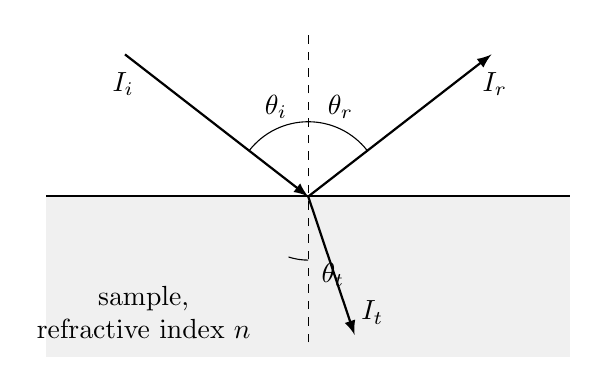
\begin{tikzpicture}[x=0.95cm,y=0.95cm,>=latex]
% interface and lower medium
\draw[thick] (-3.5,0) -- (3.5,0);
\fill[gray!12] (-3.5,-2.15) rectangle (3.5,0);
\node[align=center] at (-2.2,-1.55) {sample,\\ refractive index $n$};
% normal
\draw[dashed] (0,-1.95) -- (0,2.25);
% incident, reflected and refracted rays
\draw[->,thick] (-2.45,1.9) -- (0,0);
\node[left] at (-2.2,1.5) {$I_i$};
\draw[->,thick] (0,0) -- (2.45,1.9);
\node[right] at (2.2,1.5) {$I_r$};
\draw[->,thick] (0,0) -- (0.62,-1.85);
\node[right] at (0.58,-1.55) {$I_t$};
% angles
\draw (0,1.0) arc (90:142:1.0);
\node at (-0.43,1.2) {$\theta_i$};
\draw (0,1.0) arc (90:38:1.0);
\node at (0.43,1.2) {$\theta_r$};
\draw (0,-0.85) arc (270:252:0.85);
\node at (0.33,-1.05) {$\theta_t$};
\end{tikzpicture}
\end{figbox}

\textbf{[Apparatus and materials available]} The experimental arrangement is shown in Fig.~8.25(b).

(1) A semiconductor laser and its power supply, fixed on a rotating stage. The laser wavelength is $650\,\mathrm{nm}$.

(2) A linear polarising plate of diameter $20\,\mathrm{mm}$, fixed on a rotating stage. Note that the zero reading of the stage is not necessarily the direction of the polarisation axis of the plate.

(3) A glass plate (refractive index $1.57$ at the wavelength $650\,\mathrm{nm}$) and a thin semiconductor silicon wafer (the sample), fixed on opposite side faces of a rectangular metal block (the sample block).

(4) An optical rotating stage on which the sample block can be fixed.

(5) A digital laser power meter connected to a photodetector fixed on a support that can rotate about the sample.

(6) An optical bench, a light shield, graph paper, a flashlight, a soft tape, etc.

\begin{figbox}{8.25(b)}
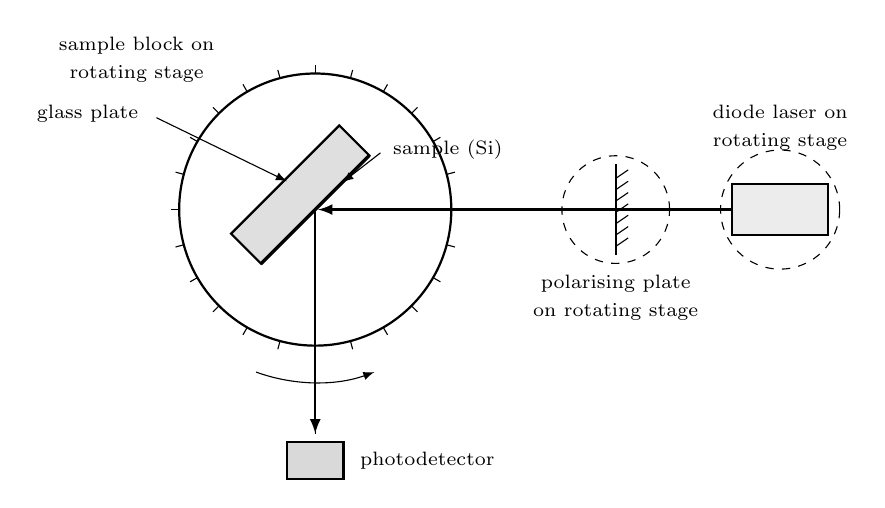
\begin{tikzpicture}[x=0.72cm,y=0.72cm,>=latex]
% sample stage
\draw[thick] (0,0) circle (2.4);
\foreach \a in {0,15,...,345} \draw (\a:2.4) -- (\a:2.55);
\node[align=center] at (-3.15,2.65) {\scriptsize sample block on\\[-2pt] \scriptsize rotating stage};
% sample block, front face through the origin, normal at -45 deg
\begin{scope}[rotate=-45]
\fill[gray!25] (-0.75,-1.35) rectangle (0,1.35);
\draw[thick] (-0.75,-1.35) rectangle (0,1.35);
\draw[very thick] (0,-1.35) -- (0,1.35);
\end{scope}
\node[right] at (1.2,1.05) {\scriptsize sample (Si)};
\draw[->] (1.15,1.0) -- (0.48,0.48);
\node[left] at (-2.95,1.7) {\scriptsize glass plate};
\draw[->] (-2.8,1.62) -- (-0.5,0.5);
% incident beam
\draw[->,thick] (8.05,0) -- (0.05,0);
% reflected beam
\draw[->,thick] (0,0) -- (0,-3.95);
% laser on its stage
\draw[thick,fill=gray!15] (7.35,-0.45) rectangle (9.05,0.45);
\draw[dashed] (8.2,0) circle (1.05);
\node[align=center] at (8.2,1.45) {\scriptsize diode laser on\\[-2pt] \scriptsize rotating stage};
% polarising plate on its stage
\draw[thick] (5.3,-0.8) -- (5.3,0.8);
\foreach \y in {-0.65,-0.45,...,0.65} \draw (5.3,\y) -- (5.52,\y+0.15);
\draw[dashed] (5.3,0) circle (0.95);
\node[align=center] at (5.3,-1.55) {\scriptsize polarising plate\\[-2pt] \scriptsize on rotating stage};
% photodetector and rotating arm
\draw[thick,fill=gray!30] (-0.5,-4.75) rectangle (0.5,-4.1);
\node[right] at (0.62,-4.42) {\scriptsize photodetector};
\draw[dashed] (0,0) -- (0,-4.1);
\draw[->] (0,0) ++(250:3.05) arc (250:290:3.05);
\end{tikzpicture}
\end{figbox}

\textbf{[Requirements]}

(1) Determine the plane of polarisation of the incident laser light. During the experiment the polarisation axis of the polarising plate should coincide with the direction of the strongest linear polarisation of the laser light.

(2) Measure the reflection coefficients $R_p$ and $R_s$ of the thin silicon wafer.

(3) Calculate the refractive index $n$ of the silicon semiconductor material.

\textbf{Solution 8.25}\quad \textbf{1.} In this experiment the plane of polarisation of the incident laser light must first be determined. Note that the light emitted by a semiconductor laser is partially polarised. To obtain the best results, the polarisation axis of the polarising plate should coincide with the strongest component of the laser light. The laser, the polarising plate and the detector are placed in a straight line. Fix either the laser or the polarising plate and rotate the other. Observe the intensity measured by the laser detector until the intensity reaches a maximum. In the subsequent measurements the polarising plate and the laser are treated as one system and are rotated together when necessary.

From the refractive index of the glass, calculate the Brewster angle of the glass from the formula
\begin{equation}
\theta_B=\arctan n \tag{4}
\end{equation}
and fix the glass sample on the rotating stage at this position. Rotate the polarisation system and measure the power of the reflected laser light at different polarisation angles. The experimental results are shown in Fig.~8.25(c). From this the orientation of the polarising plate, relative to the glass sample, at which the reflected laser power is minimum can be found. According to Brewster's principle, it can be determined that at this position the plane of polarisation of the laser light is parallel to the plane of incidence on the sample.

\begin{figbox}{8.25(c)}
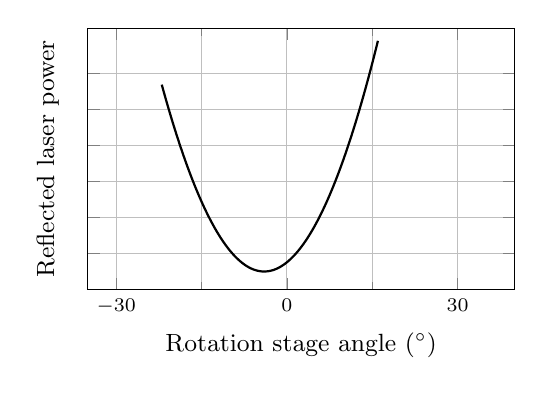
\begin{tikzpicture}
\begin{axis}[
  width=7.0cm, height=4.9cm,
  xlabel={Rotation stage angle ($^\circ$)},
  ylabel={Reflected laser power},
  xmin=-35, xmax=40, ymin=0, ymax=1.45,
  xtick={-30,0,30},
  ytick={0.2,0.4,...,1.2},
  yticklabels={},
  grid=both,
  minor x tick num=1,
  tick label style={font=\scriptsize},
  label style={font=\small},
  axis line style={-},
]
\addplot[domain=-22:16,samples=120,thick] {0.10+0.0032*(x+4)^2};
\end{axis}
\end{tikzpicture}
\end{figbox}

\textbf{2.} With the direction of the laser polarisation plane determined above, make it respectively perpendicular and parallel to the plane of incidence on the silicon semiconductor, and measure the reflected laser power at different angles, as shown in Fig.~8.25(d). In this figure the relations $R_p$--$\theta_i$ and $R_s$--$\theta_i$, extrapolated to zero angle of incidence $\theta_i$, should meet at one point.

When plotting, note that more points should be measured near the minimum so as to ensure the smoothness and correctness of the graph.

\begin{figbox}{8.25(d)}
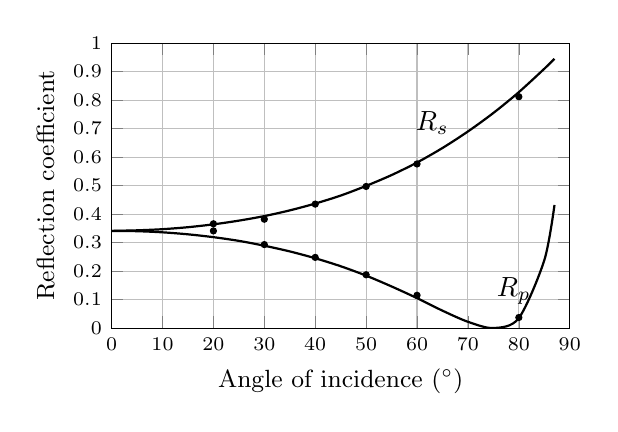
\begin{tikzpicture}
\begin{axis}[
  width=7.4cm, height=5.2cm,
  xlabel={Angle of incidence ($^\circ$)},
  ylabel={Reflection coefficient},
  xmin=0, xmax=90, ymin=0, ymax=1.0,
  xtick={0,10,...,90},
  ytick={0,0.1,...,1.0},
  grid=both,
  tick label style={font=\scriptsize},
  label style={font=\small},
  axis line style={-},
]
\addplot[thick,smooth] coordinates {
(0,0.341) (5,0.343) (10,0.347) (15,0.354) (20,0.364) (25,0.377)
(30,0.393) (35,0.413) (40,0.437) (45,0.465) (50,0.499) (55,0.537)
(60,0.581) (65,0.632) (70,0.690) (75,0.755) (80,0.828) (85,0.910) (87,0.945)};
\node at (axis cs:63,0.72) {$R_s$};
\addplot[thick,smooth] coordinates {
(0,0.341) (5,0.340) (10,0.336) (15,0.329) (20,0.319) (25,0.306)
(30,0.289) (35,0.269) (40,0.245) (45,0.217) (50,0.184) (55,0.146)
(60,0.105) (65,0.061) (70,0.022) (75,0.000) (80,0.035) (85,0.238) (87,0.432)};
\node at (axis cs:79,0.13) {$R_p$};
\addplot[only marks,mark=*,mark size=1.1pt] coordinates {
(20,0.366) (30,0.382) (40,0.435) (50,0.497) (60,0.576) (80,0.812)};
\addplot[only marks,mark=*,mark size=1.1pt] coordinates {
(20,0.341) (30,0.293) (40,0.248) (50,0.187) (60,0.115) (80,0.037)};
\end{axis}
\end{tikzpicture}
\end{figbox}

\textbf{3.} The average values of several measurements of the refractive index are shown in the following table.

\begin{center}
\textbf{Table 8.25}\\[3pt]
\begin{tabular}{ccccc}
\toprule
$\theta_i/\degree$ & $R_p$ & $R_s$ & $n$ & $\bar{n}$ \\
\midrule
20.0 & 0.341 & 0.366 & 3.93 & \\
30.0 & 0.293 & 0.382 & 3.82 & \\
40.0 & 0.248 & 0.435 & 3.81 & \\
50.0 & 0.187 & 0.497 & 3.82 & \\
60.0 & 0.115 & 0.576 & 3.85 & \\
80.0 & 0.037 & 0.812 & 3.61 & \\
\midrule
\multicolumn{4}{r}{Average} & 3.81 \\
\bottomrule
\end{tabular}
\end{center}

\begin{commentary}
This problem is an optics experimental problem from the 3rd Asian Physics Olympiad. The experiment requires students to master thoroughly the theory of polarised light and the operational skills of experimental adjustment; in addition, more points should be measured near the extremum so that this problem can be done well.
\end{commentary}

\subsection*{Experiment 8.26 \quad Measurement of the refractive index of glass by the Brewster-angle method}

\textbf{[Apparatus and materials available]} Spectrometer, helium--neon laser with polarised output, polarising plate with an angular scale, prism under test, white screen, etc.

\textbf{[Requirements]}

(1) Write down the principle of the experiment and the experimental formula.

(2) Draw a simple diagram of the experiment.

(3) Measure the experimental data and calculate the result.

(4) Estimate the experimental error.

\textbf{Solution 8.26}\quad \textbf{1.} A beam of plane-polarised light of wavelength $\lambda$ whose electric vector is parallel to the plane of incidence (called a TM wave) is incident from air at the Brewster angle $i_B$ on the surface of a medium of refractive index $n$. At this interface the reflection coefficient of the TM wave is zero, and the incident light enters the medium completely. According to Brewster's law, the tangent of the angle of incidence $i_B$ is equal to the refractive index $n$ of the medium at the wavelength $\lambda$, that is,
\begin{equation}
\tan i_B=n. \tag{1}
\end{equation}
It follows that if the angle of incidence of the TM wave is varied, the Brewster angle can be determined when the intensity of the reflected light is zero, and the refractive index of the optical medium under test follows from formula (1).

\textbf{2.} As shown in the figure, the prism is placed vertically on the small platform of the spectrometer. The laser light, whose polarisation has been adjusted beforehand---that is, plane-polarised light whose electric vector is incident at a certain angle---is reflected from the glass surface, and the reflected light is followed with an analyser, so that the intensity of the reflected light can be observed on the white screen. During the experiment the analyser must be rotated continuously in order to observe the state of the reflected polarisation. If the turntable of the spectrometer is rotated to change the angle of incidence of the laser light, and the analyser and the turntable are adjusted carefully, then when the intensity of the reflected light passing through the analyser on the white screen is zero, the reading can be taken from the spectrometer and the Brewster angle $i_B$ determined.

\begin{figbox}{8.26}
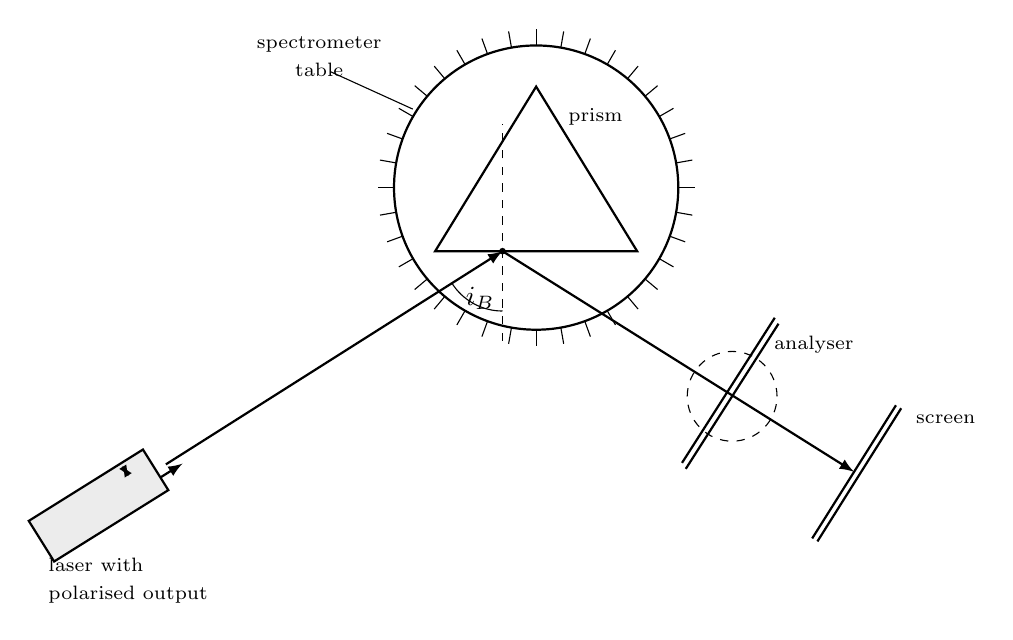
\begin{tikzpicture}[x=0.95cm,y=0.95cm,>=latex]
% spectrometer table
\draw[thick] (0,0.5) circle (1.9);
\foreach \a in {0,10,...,350} \draw (0,0.5) ++(\a:1.9) -- ++(\a:0.22);
\node[align=center] at (-2.9,2.25) {\scriptsize spectrometer\\[-2pt] \scriptsize table};
\draw (-2.75,2.05) -- (-1.65,1.55);
% prism
\coordinate (A) at (0,1.85);
\coordinate (B) at (-1.35,-0.35);
\coordinate (C) at (1.35,-0.35);
\draw[thick] (A) -- (B) -- (C) -- cycle;
\node[right] at (0.3,1.45) {\scriptsize prism};
% point of incidence on the lower face
\coordinate (P) at (-0.45,-0.35);
\fill (P) circle (1.2pt);
% normal
\draw[dashed] (-0.45,-1.55) -- (-0.45,1.35);
% incident beam from the laser
\draw[->,thick] (-4.95,-3.2) -- (P);
% reflected beam
\draw[->,thick] (P) -- (4.25,-3.3);
% laser
\begin{scope}[shift={(-5.85,-3.75)},rotate=32]
\draw[thick,fill=gray!15] (-0.9,-0.32) rectangle (0.9,0.32);
\draw[->,thick] (0.9,-0.12) -- (1.25,-0.12);
\draw[<->] (0.55,0.12) -- (0.55,0.28);
\end{scope}
\node[align=left,anchor=north west] at (-6.65,-4.32) {\scriptsize laser with\\[-2pt] \scriptsize polarised output};
% analyser, perpendicular to the reflected beam
\coordinate (Q) at (2.62,-2.29);
\draw[dashed] (Q) circle (0.6);
\draw[thick] (3.24,-1.32) -- (2.00,-3.26);
\draw[thick] (3.19,-1.24) -- (1.95,-3.18);
\node[right] at (3.05,-1.6) {\scriptsize analyser};
% screen, perpendicular to the reflected beam
\coordinate (S) at (4.25,-3.3);
\draw[thick] (4.81,-2.41) -- (3.69,-4.19);
\draw[thick] (4.88,-2.45) -- (3.76,-4.23);
\node[right] at (4.95,-2.6) {\scriptsize screen};
% Brewster angle
\draw (P) ++(212:0.8) arc (212:270:0.8);
\node at (-0.75,-0.98) {$i_B$};
\end{tikzpicture}
\end{figbox}

\textbf{3. Experimental results and error calculation}

The measured Brewster angle is $i_B=57\degree0'$, so the refractive index is
\[
n=\tan 57\degree0'=1.54.
\]
From $n=\tan i_B$, $\Delta i_B$ is estimated to be $0.5\degree$, that is, $\Delta i_B=\frac{\pi}{360}=0.009$.

\[
\Delta n=\Delta(\tan i_B)=\frac{\Delta i_B}{(\cos i_B)^2}
=\frac{0.009}{(\cos 57\degree0')^2}=\frac{0.009}{0.297}=0.03.
\]
Therefore the refractive index of the glass is $n=1.54\pm0.03$.
